% Options for packages loaded elsewhere
\PassOptionsToPackage{unicode}{hyperref}
\PassOptionsToPackage{hyphens}{url}
%
\documentclass[
  man,floatsintext]{apa7}
\usepackage{amsmath,amssymb}
\usepackage{iftex}
\ifPDFTeX
  \usepackage[T1]{fontenc}
  \usepackage[utf8]{inputenc}
  \usepackage{textcomp} % provide euro and other symbols
\else % if luatex or xetex
  \usepackage{unicode-math} % this also loads fontspec
  \defaultfontfeatures{Scale=MatchLowercase}
  \defaultfontfeatures[\rmfamily]{Ligatures=TeX,Scale=1}
\fi
\usepackage{lmodern}
\ifPDFTeX\else
  % xetex/luatex font selection
\fi
% Use upquote if available, for straight quotes in verbatim environments
\IfFileExists{upquote.sty}{\usepackage{upquote}}{}
\IfFileExists{microtype.sty}{% use microtype if available
  \usepackage[]{microtype}
  \UseMicrotypeSet[protrusion]{basicmath} % disable protrusion for tt fonts
}{}
\makeatletter
\@ifundefined{KOMAClassName}{% if non-KOMA class
  \IfFileExists{parskip.sty}{%
    \usepackage{parskip}
  }{% else
    \setlength{\parindent}{0pt}
    \setlength{\parskip}{6pt plus 2pt minus 1pt}}
}{% if KOMA class
  \KOMAoptions{parskip=half}}
\makeatother
\usepackage{xcolor}
\usepackage{graphicx}
\makeatletter
\newsavebox\pandoc@box
\newcommand*\pandocbounded[1]{% scales image to fit in text height/width
  \sbox\pandoc@box{#1}%
  \Gscale@div\@tempa{\textheight}{\dimexpr\ht\pandoc@box+\dp\pandoc@box\relax}%
  \Gscale@div\@tempb{\linewidth}{\wd\pandoc@box}%
  \ifdim\@tempb\p@<\@tempa\p@\let\@tempa\@tempb\fi% select the smaller of both
  \ifdim\@tempa\p@<\p@\scalebox{\@tempa}{\usebox\pandoc@box}%
  \else\usebox{\pandoc@box}%
  \fi%
}
% Set default figure placement to htbp
\def\fps@figure{htbp}
\makeatother
\setlength{\emergencystretch}{3em} % prevent overfull lines
\providecommand{\tightlist}{%
  \setlength{\itemsep}{0pt}\setlength{\parskip}{0pt}}
\setcounter{secnumdepth}{-\maxdimen} % remove section numbering
% Make \paragraph and \subparagraph free-standing
\makeatletter
\ifx\paragraph\undefined\else
  \let\oldparagraph\paragraph
  \renewcommand{\paragraph}{
    \@ifstar
      \xxxParagraphStar
      \xxxParagraphNoStar
  }
  \newcommand{\xxxParagraphStar}[1]{\oldparagraph*{#1}\mbox{}}
  \newcommand{\xxxParagraphNoStar}[1]{\oldparagraph{#1}\mbox{}}
\fi
\ifx\subparagraph\undefined\else
  \let\oldsubparagraph\subparagraph
  \renewcommand{\subparagraph}{
    \@ifstar
      \xxxSubParagraphStar
      \xxxSubParagraphNoStar
  }
  \newcommand{\xxxSubParagraphStar}[1]{\oldsubparagraph*{#1}\mbox{}}
  \newcommand{\xxxSubParagraphNoStar}[1]{\oldsubparagraph{#1}\mbox{}}
\fi
\makeatother
% definitions for citeproc citations
\NewDocumentCommand\citeproctext{}{}
\NewDocumentCommand\citeproc{mm}{%
  \begingroup\def\citeproctext{#2}\cite{#1}\endgroup}
\makeatletter
 % allow citations to break across lines
 \let\@cite@ofmt\@firstofone
 % avoid brackets around text for \cite:
 \def\@biblabel#1{}
 \def\@cite#1#2{{#1\if@tempswa , #2\fi}}
\makeatother
\newlength{\cslhangindent}
\setlength{\cslhangindent}{1.5em}
\newlength{\csllabelwidth}
\setlength{\csllabelwidth}{3em}
\newenvironment{CSLReferences}[2] % #1 hanging-indent, #2 entry-spacing
 {\begin{list}{}{%
  \setlength{\itemindent}{0pt}
  \setlength{\leftmargin}{0pt}
  \setlength{\parsep}{0pt}
  % turn on hanging indent if param 1 is 1
  \ifodd #1
   \setlength{\leftmargin}{\cslhangindent}
   \setlength{\itemindent}{-1\cslhangindent}
  \fi
  % set entry spacing
  \setlength{\itemsep}{#2\baselineskip}}}
 {\end{list}}
\usepackage{calc}
\newcommand{\CSLBlock}[1]{\hfill\break\parbox[t]{\linewidth}{\strut\ignorespaces#1\strut}}
\newcommand{\CSLLeftMargin}[1]{\parbox[t]{\csllabelwidth}{\strut#1\strut}}
\newcommand{\CSLRightInline}[1]{\parbox[t]{\linewidth - \csllabelwidth}{\strut#1\strut}}
\newcommand{\CSLIndent}[1]{\hspace{\cslhangindent}#1}
\ifLuaTeX
\usepackage[bidi=basic]{babel}
\else
\usepackage[bidi=default]{babel}
\fi
\babelprovide[main,import]{english}
% get rid of language-specific shorthands (see #6817):
\let\LanguageShortHands\languageshorthands
\def\languageshorthands#1{}
\ifLuaTeX
  \usepackage[english]{selnolig} % disable illegal ligatures
\fi
% Manuscript styling
\usepackage{upgreek}
\captionsetup{font=singlespacing,justification=justified}

% Table formatting
\usepackage{longtable}
\usepackage{lscape}
% \usepackage[counterclockwise]{rotating}   % Landscape page setup for large tables
\usepackage{multirow}		% Table styling
\usepackage{tabularx}		% Control Column width
\usepackage[flushleft]{threeparttable}	% Allows for three part tables with a specified notes section
\usepackage{threeparttablex}            % Lets threeparttable work with longtable

% Create new environments so endfloat can handle them
% \newenvironment{ltable}
%   {\begin{landscape}\centering\begin{threeparttable}}
%   {\end{threeparttable}\end{landscape}}
\newenvironment{lltable}{\begin{landscape}\centering\begin{ThreePartTable}}{\end{ThreePartTable}\end{landscape}}

% Enables adjusting longtable caption width to table width
% Solution found at http://golatex.de/longtable-mit-caption-so-breit-wie-die-tabelle-t15767.html
\makeatletter
\newcommand\LastLTentrywidth{1em}
\newlength\longtablewidth
\setlength{\longtablewidth}{1in}
\newcommand{\getlongtablewidth}{\begingroup \ifcsname LT@\roman{LT@tables}\endcsname \global\longtablewidth=0pt \renewcommand{\LT@entry}[2]{\global\advance\longtablewidth by ##2\relax\gdef\LastLTentrywidth{##2}}\@nameuse{LT@\roman{LT@tables}} \fi \endgroup}

% \setlength{\parindent}{0.5in}
% \setlength{\parskip}{0pt plus 0pt minus 0pt}

% Overwrite redefinition of paragraph and subparagraph by the default LaTeX template
% See https://github.com/crsh/papaja/issues/292
\makeatletter
\renewcommand{\paragraph}{\@startsection{paragraph}{4}{\parindent}%
  {0\baselineskip \@plus 0.2ex \@minus 0.2ex}%
  {-1em}%
  {\normalfont\normalsize\bfseries\itshape\typesectitle}}

\renewcommand{\subparagraph}[1]{\@startsection{subparagraph}{5}{1em}%
  {0\baselineskip \@plus 0.2ex \@minus 0.2ex}%
  {-\z@\relax}%
  {\normalfont\normalsize\itshape\hspace{\parindent}{#1}\textit{\addperi}}{\relax}}
\makeatother

\makeatletter
\usepackage{etoolbox}
\patchcmd{\maketitle}
  {\section{\normalfont\normalsize\abstractname}}
  {\section*{\normalfont\normalsize\abstractname}}
  {}{\typeout{Failed to patch abstract.}}
\patchcmd{\maketitle}
  {\section{\protect\normalfont{\@title}}}
  {\section*{\protect\normalfont{\@title}}}
  {}{\typeout{Failed to patch title.}}
\makeatother

\usepackage{xpatch}
\makeatletter
\xapptocmd\appendix
  {\xapptocmd\section
    {\addcontentsline{toc}{section}{\appendixname\ifoneappendix\else~\theappendix\fi: #1}}
    {}{\InnerPatchFailed}%
  }
{}{\PatchFailed}
\makeatother
\keywords{numeracy, judgments, memory, expertise}
\usepackage{lineno}

\linenumbers
\usepackage{csquotes}
\makeatletter
\renewcommand{\paragraph}{@startsection{paragraph}{4}{\parindent}%
  {0\baselineskip @plus 0.2ex @minus 0.2ex}%
  {-1em}%
  {\normalfont\normalsize\bfseries\typesectitle}}

\renewcommand{\subparagraph}[1]{@startsection{subparagraph}{5}{1em}%
  {0\baselineskip @plus 0.2ex @minus 0.2ex}%
  {-\z@\relax}%
  {\normalfont\normalsize\bfseries\itshape\hspace{\parindent}{#1}\textit{\addperi}}{\relax}}
\makeatother

\usepackage{bookmark}
\IfFileExists{xurl.sty}{\usepackage{xurl}}{} % add URL line breaks if available
\urlstyle{same}
\hypersetup{
  pdftitle={Counting on Memory: How Expertise Shapes Our Numerical Judgments of Associations},
  pdfauthor={Erin M. Buchanan1},
  pdflang={en-EN},
  pdfkeywords={numeracy, judgments, memory, expertise},
  hidelinks,
  pdfcreator={LaTeX via pandoc}}

\title{Counting on Memory: How Expertise Shapes Our Numerical Judgments of Associations}
\author{Erin M. Buchanan\textsuperscript{1}}
\date{}


\shorttitle{COUNTING MEMORY}

\authornote{

Correspondence concerning this article should be addressed to Erin M. Buchanan, 326 Market St., Harrisburg, PA 17101. E-mail: \href{mailto:ebuchanan@harrisburgu.edu}{\nolinkurl{ebuchanan@harrisburgu.edu}}

}

\affiliation{\vspace{0.5cm}\textsuperscript{1} Harrisburg University of Science and Technology}

\abstract{%
Accurate numerical estimation underlies many aspects of cognition, from basic quantity judgments to complex decision-making. One domain where numerical reasoning is especially critical is memory, where individuals often must estimate the likelihood that one event or idea is associated with another. In this study, participants completed a free association task across multiple sessions to generate their own individualized word-pair norms. Later, they provided numerical probability judgments (0--100\%) of how often they had produced each pair. These judgments were compared to collective free association norms, a matched group evaluating others' pairs, and a traditional control group. Results showed that participants who judged their own pairs were significantly more accurate in estimating associative probabilities than control or matched groups, reflecting the benefits of expertise derived from repeated interaction with stimuli. However, systematic overestimation bias persisted, especially for weak associations, indicating that metacognitive sensitivity to probability differences remains limited. These findings highlight how expertise improves---but does not perfect---the ability to translate memory associations into numerical judgments, offering new insights into the intersection of numerical cognition, metacognition, and memory.
}



\begin{document}
\maketitle

People are often asked to make numerical judgments of frequency or
probability in daily life. For instance, if you are waiting for a friend
who is late to lunch, you must estimate whether lateness is a
high-frequency or low-frequency event to decide when to become
concerned. Such numerical judgments are prone to systematic bias, and
research has long shown that people tend to inflate their estimates in
many domains. In education, for example, students often judge their
competence at levels higher than their actual performance supports
(Dunning et al., 2003). Similarly, judgments of learning (JOLs) are typically
overconfident, which can lead to inefficient study strategies
(Koriat \& Bjork, 2005). Individuals who self-monitor their study habits are
frequently highly confident but poorly calibrated in their learning
(Cutler \& Wolfe, 1989). These findings point to a broader problem in cognition:
people struggle to map memory experiences onto accurate numerical
estimates, underscoring the need for methods that remediate inflated
predictions for both theoretical and applied purposes (Koriat, 2008; Koriat \& Bjork, 2006). This issue resonates with central questions in numerical
cognition, where researchers investigate how humans perceive and
evaluate numerical magnitudes, probabilities, and quantities
(Dehaene, 2011; Reyna \& Brainerd, 2008).

Word associations provide a rich domain for studying how people generate
and evaluate numerical judgments of probability, making them a useful
context for investigating inflated predictions and their potential
remediation (Koriat \& Bjork, 2006; Maki, 2007a). Typically, word associations are
measured using the method of free association (Nelson et al., 2000), in which
participants provide the first word (target) that comes to mind when
presented with another word (cue). When aggregated across many
individuals, the likelihood that word B follows word A, termed the
forward strength (FSG), is expressed as a conditional probability, a
fundamentally numerical index of associative strength. Large-scale
databases now provide probabilistic values for thousands of cue--response
pairs (De Deyne et al., 2019; Nelson et al., 2004). For example, the probability that
\emph{computer} elicits the response \emph{program} is approximately 12\%, meaning
that about 12 of 100 people produce that pairing. Thus, free association
tasks translate linguistic memory associations into numerical
probability values, making them an ideal bridge between memory research
and numerical cognition.

Studies of inflated predictions in word associations consistently show
that people overestimate the numerical probability of word relations,
particularly for weakly associated pairs (Maki, 2007b). This inflation
effect represents a systematic bias in probability estimation,
paralleling findings in broader numerical cognition where people often
misjudge small magnitudes or low-probability events (e.g., Gigerenzer \& Hoffrage, 1995; Reyna \& Brainerd, 2008). The tendency toward assigning excessively
high ratings is remarkably resistant to change (Maki, 2007a; Nelson et al., 2005; Valentine \& Buchanan, 2013). For example, the inflation persists even
when participants are provided with a list of common associates for a
given cue (Foster \& Buchanan, 2012), when they are prompted to consider alternative
responses (Maki, 2007a), or even when they overtly generate their own
list of associates (Koriat, 2008; Koriat \& Bjork, 2006). In all these cases,
numerical judgments of associative probability remain poorly calibrated,
underscoring the robustness of estimation bias across both memory and
numerical domains.

Because of the robustness of the inflation effect, finding ways to
reduce it is important. Prior work has shown that mnemonic and
theory-based debiasing procedures can reduce overall overestimation
bias, but these methods rarely improve sensitivity: the ability to
discriminate between low- and high-probability events (Valentine \& Buchanan, 2013).
In terms of numerical cognition, \emph{bias} reflects a systematic tendency
to assign inflated probability values (treating most associations as
stronger than they truly are), whereas \emph{sensitivity} reflects accuracy
in tuning numerical judgments to actual associative strength
(Maki, 2007a). The current experiment tested whether using individually
normed frequencies would improve numerical estimation of associative
probabilities. Previous studies have shown that people are generally
poor at estimating what \emph{others} would say when given a particular cue
word (Buchanan, 2010; Foster \& Buchanan, 2012; Maki, 2007a, 2007b; Maxwell \& Buchanan, 2020; Maxwell \& Huff, 2021), suggesting that collective norms are difficult to
approximate. In a traditional judgment of associative memory (JAM) task,
participants estimate how many people out of 100 would produce a target
word in response to a cue (Maki, 2007b). In contrast, our design had
participants generate their own frequency norms across multiple sessions
and then judge the probability of their own cue--target pairings. If
these frequency memories function like distributed practice in study
skills, repeated exposure should foster expertise in probability
estimation, improving judgment capacity relative to comparison groups.

The following hypotheses were examined:

\begin{itemize}
\tightlist
\item
  \emph{Hypothesis 1}: Individual normed cue-response probabilities will be
  correlated with previous database probabilities on an individual and
  overall participant level.
\item
  \emph{Hypothesis 2}: Free association database norms will be predictive
  of all group's judgments. Mixed linear models will be used to
  calculate the slope of judgments when compared to free association
  norms. Given previous research (Maki, 2007b, 2007a; Valentine \& Buchanan, 2013), the values were expected to be sensitive (\emph{b} \(\ne\)

  \begin{enumerate}
  \def\labelenumi{\arabic{enumi})}
  \setcounter{enumi}{-1}
  \tightlist
  \item
    but not perfectly attuned (\emph{b} = 1).
  \end{enumerate}
\item
  \emph{Hypothesis 3}: Judgment ability will vary across groups, so that
  the experimental group should show better judgment ability when
  compared to their own norms over control, matched, and experimental
  groups compared to free association norms.
\end{itemize}

These hypotheses underscore how expertise, operationalized as repeated
interaction with specific word pairings and their frequencies, affects
the ability to make numerical judgments of probability from memory. In
studies of distributed practice, repeated exposure increases the
subjective likelihood of remembering an item, leading to higher
judgments of learning. A parallel process can be expected here: as items
are encountered repeatedly, participants should assign higher
probability values to those associations, reflecting strengthened memory
connections. Thus, expertise not only improves memory retention but also
has the potential to enhance the calibration of numerical estimates,
linking metacognitive monitoring with fundamental processes in numerical
cognition.

\section{Method}\label{method}

\subsection{Participants}\label{participants}

Participants were recruited through the Department of Psychology's
undergraduate subject pool at a large Midwestern university. Students
were required to participate in research for their general psychology
course, and some upper-level courses allowed research participation for
extra credit. The research project was displayed on the SONA system, an
online participant-credit management platform, and participants selected
studies to complete based on availability and interest in the posted
abstract. The entire experiment was completed online, with each section
lasting approximately five to fifteen minutes. In the experimental
group, \emph{n} = 51 participants began the study, with \emph{n} = 41
completing all experimental sessions. For the non-finishing group (\emph{n} =
14), the average number of sessions was \emph{M} = 2.14 (\emph{SD} = 1.17), with a
range of one to four rating sessions. The comparison groups included
52 participants for the control group and
41 participants for the matched group.

\subsection{Materials}\label{materials}

Stimuli were selected from the free association word norms by
Nelson et al. (2004). The database includes a list of cues shown to participants,
with the responses given by participants in their study. For example,
with the pair \emph{steak-sirloin}, \emph{steak} is the cue word that is paired
with the target word, \emph{sirloin}. Each cue word (the first word) has
several different target words (\emph{steak-cow}, \emph{steak-sauce}). Cue words
were selected with varying number of target combinations, specifically,
ten cue words with small cue set sizes and ten cues with large cue set
sizes. Cue set size indicates the number of other pairs in the database;
for example, \emph{car} has 25 cue-target combinations in the Nelson et al. (2004)
database, while \emph{pupil} only has four cue-target combinations.

The forward strength (FSG) indicates the likelihood of the the response,
given the cue (\(P(response|cue)\)), while backward strength (BSG)
indicates the reverse probability (\(P(cue|response\))). Free association
probability is not symmetric, and therefore, FSG \(\ne\) BSG in most
cue-response pairs. The ten cue words with a smaller cue set size
(\(M_{Set Size}\) = 4.10, \(SD_{Set Size}\) =
0.63, range = 3-5) had an average forward strength
of \(M_{FSG}\) = .23 (\(SD_{FSG}\) =
.30) and backward strength of \(M_{BSG}\) =
.03 (\emph{SD} =
.09). The larger cue set size words
(\(M_{Set Size}\) = 24.96, \(SD_{Set Size}\) =
4.35, range = 20-33) had a forward strength of
\(M_{FSG}\) = .03 (\(SD_{FSG}\) =
.03) and a backwards strength of \(M_{BSG}\)
= .05 (\(SD_{BSG}\) =
.11). Target word selection is described
below. The complete set of materials can be found at
\url{https://github.com/doomlab/jam-numeracy-longitudinal}.

\subsection{Procedure}\label{procedure}

\subsubsection{Experimental Group}\label{experimental-group}

\textbf{Norming Phase.}

This group of participants was given the opportunity to compare their
own pairing probabilities rather than estimating others' likely
judgments. In the norming stage, participants received instructions for
a free association task, described as writing down ``the first word that
pops into your mind when you hear a cue word.'' For example, many people
may associate \emph{cat} with \emph{dog} because of common ownership, but they may
also produce idiomatic responses such as it's raining cats and dogs.
These examples emphasized free association as reflecting general
language use rather than limited to literal features (e.g., \emph{fur},
\emph{tails}, \emph{whiskers}). After these instructions, participants were
presented with twenty cue words, each accompanied by four blanks. For
each cue word, they wrote the first four target words that came to mind,
providing variation in the target responses during the initial stage.
All responses were stored for later use.

After a minimum delay of two days, participants were invited to complete
the survey again. Email reminders were sent when the next session became
available. Each participant completed the survey five times, with cue
words randomized at each presentation. Responses across the five
sessions were then averaged to generate probabilities for each
cue--target pairing, following procedures similar to those used in the
free association database (Nelson et al., 2004). For example, across five
sessions, a participant might generate several different responses to
the cue \emph{computer}, such as \emph{mouse}, \emph{screen}, \emph{game}, \emph{program},
\emph{keyboard}, or \emph{data}. Each cue--target probability reflected the
proportion of sessions in which that target was produced (e.g., if
screen was listed in all five sessions, its probability was 5/5, or
100\%). From these data, 50 cue--target combinations were selected for
each participant, with ten word--target pairs drawn from each probability
level (20\%, 40\%, 60\%, 80\%, and 100\%).

\textbf{Judgment Phase.}

Participants were then asked to estimate the probability of each of
their cue--target combinations. For example, a participant might see the
prompt: ``When asked about \emph{computer}, you listed the word \emph{program}.
What percent of the time did you put computer and program together?''
Responses were made on a rating scale with five options (20\%, 40\%, 60\%,
80\%, and 100\%) by selecting the appropriate radio button. After
completing the final survey, participants were debriefed.The complete
dataset of cue--target responses and probability judgments from both
phases, along with an R Markdown analysis file created using the
\emph{papaja} package (Aust et al., 2022), is available at our GitHub repository:
\url{https://github.com/doomlab/jam-numeracy-longitudinal}.

\subsubsection{Control Group}\label{control-group}

Results from a separate control group were compared with the
experimental participants' judgment scores. Because each experimental
participant's final word pairs were unique, a set of cue--target pairings
was selected from the free association database (Nelson et al., 2004) to serve
as a comparison. The same twenty cue words were used, with target words
chosen to ensure an equal distribution of low-, medium-, and
high-strength associations. For each cue word from the experimental
norming phase, three cue--target pairs were selected, yielding a total of
60 word pairs. Several cues were necessarily repeated to create the full
set of 60 pairs, thereby matching the repetition structure used in the
experimental group. The average FSG was \emph{M} =
0.00 (\emph{SD} =
0.00) and the BSG was \emph{M} =
0.08 (\emph{SD} =
0.15). The control group was
given the same instructions about a free association task, along with
examples.Next, the rating task was explained as follows: ``How many
people out of a 100 would give the target (second) word when asked the
cue (first) word?'' Participants estimated the probability of word pair
occurrence using the same 20\%-40\%-60\%-80\%-100\% scale as the experimental
group.

\subsubsection{Control Matched Group}\label{control-matched-group}

Last, a separate comparison group was included to parallel the
experimental group. Each participant in this group was randomly paired
with an experimental participant. They received the same instructions as
the control group for both the free association and rating tasks.
However, rather than judging randomly selected word--pairs, they
evaluated the normed word--pairs generated by their paired experimental
participant. This matched group provided a test of stimulus effects on
judgment, allowing us to determine whether improved performance in the
experimental group was specifically due to participants' prior
interaction with the word--pairs.

\section{Results}\label{results}

\subsection{Experimental Norming Descriptive Statistics}\label{experimental-norming-descriptive-statistics}

The data were split into separate cue-response combinations for each
participant and norming time point. Response were spelled checked and
corrected unless the answer was not obvious or was a combination of
prefixes and regular words (e.g., \emph{un-special}). Determinants (\emph{the, an,
a}) and other stopwords were removed from the responses (\emph{of, to, than,
that, then, so, if, too, or, as}). Words were not lemmatized and were
left in their original form (e.g., \emph{arm} and \emph{arms} were left separate).
If a participant listed a response word more than once per session for a
cue, it was deleted, so that the maximum number of times a cue-response
pair could be mentioned was five times.

Across all five testing sessions, participants generated a large and
varied set of responses. On average, each participant listed \emph{M} =
190.61 (\emph{SD} =
42.72) unique
response words, resulting in a total of 8687 cue--response
pairs across the experiment after removal of the stopwords and filler
words. The vast majority of responses were produced only once per
participant (\emph{n} = 5180), demonstrating that participants
were not simply repeating a small set of highly accessible words, but
instead generating a broad range of associations across sessions. At the
same time, a smaller set was observed in four or five responses (\emph{n} =
1415), indicating that a subset of cue--response pairs were
consistently retrieved across most sessions and reflected particularly
strong associations. This dual pattern, mostly novel responses, with a
small cluster of repeated pairings, captures both the flexibility and
stability of associative memory.

At the stimulus level, cues elicited an average of \emph{M} =
184.25 (\emph{SD} =
33.88) unique targets,
underscoring the diversity of responses to each word. When collapsed
across all participants and stimuli, the experiment yielded
2555 distinct
target words. This broad distribution suggests that free association
tasks elicit a wide variety of lexical connections, while the consistent
recurrence of certain responses highlights the emergence of
high-frequency, strongly linked associations. Together, these
descriptive findings show that the experimental design successfully
captured both the variability of associative networks and the stability
of robust word pairings, setting the stage for later analyses of
participants' probability judgments.

\subsection{Hypothesis 1}\label{hypothesis-1}

These cue--response pairs were merged with the Nelson et al. (2004) and
De Deyne et al. (2019) free association norms. The 3685 unique
cue--response pairs across all participants in the experimental norming
group overlapped with the Nelson et al. (2004) norms by
6.46\% and with the
De Deyne et al. (2019) norms by 26.78\%.

To test how closely participant ratings tracked normative values, we fit
mixed linear models that accounted for repeated measurements within
participants and correlated error structures (Gelman, 2006). Each model
included a random intercept for participant and random slopes for
forward strength, allowing us to estimate individual differences in both
overall bias and sensitivity. Using the \emph{nlme} package in \emph{R}, fixed
effects were specified as database values predicting participant
response frequencies, with all predictors normalized to the same scale.
As shown in Figure \ref{fig:fig-fsg-swow-scores}, participant judgments
were positively related to both sets of normative values. A perfect
calibration would correspond to an intercept of 0 (no upward bias, Maki, 2007b) and a slope of 1 (perfect sensitivity). Given the
individualized nature of our norms and the fact that the design
precludes true zero ratings, we expected some upward bias in intercepts,
but slopes greater than zero would indicate sensitivity to associative
strength (\(b \ne 0\)).

For the Nelson et al. (2004) data, the intercept showed an upward bias,
\(\hat{\beta} = 0.45\), 95\% CI \([0.43, 0.47]\),
\(t(2180) = 37.14\), \(p < .001\), and the slope was significantly
different from zero, \(\hat{\beta} = 0.53\), 95\% CI \([0.48, 0.59]\),
\(t(2180) = 19.29\), \(p < .001\). Random effects revealed variability
across participants, with \emph{SD} = 0.06 for intercepts and \emph{SD} = 0.09 for
slopes. For the De Deyne et al. (2019) (SWOW) data, intercept bias was smaller,
\(\hat{\beta} = 0.38\), 95\% CI \([0.36, 0.39]\),
\(t(4891) = 39.81\), \(p < .001\), and slope sensitivity was
higher than with Nelson norms, \(\hat{\beta} = 0.73\), 95\% CI \([0.68, 0.79]\),
\(t(4891) = 26.03\), \(p < .001\). Variability was again evident, with
random intercept \emph{SD} = 0.05 and random slope \emph{SD} = 0.12. Together,
these results indicate that participants' probability judgments reliably
tracked normative association strength, with evidence for both upward
bias and meaningful individual differences in sensitivity, consistent
with Hypothesis 1.

\begin{figure}
\centering
\pandocbounded{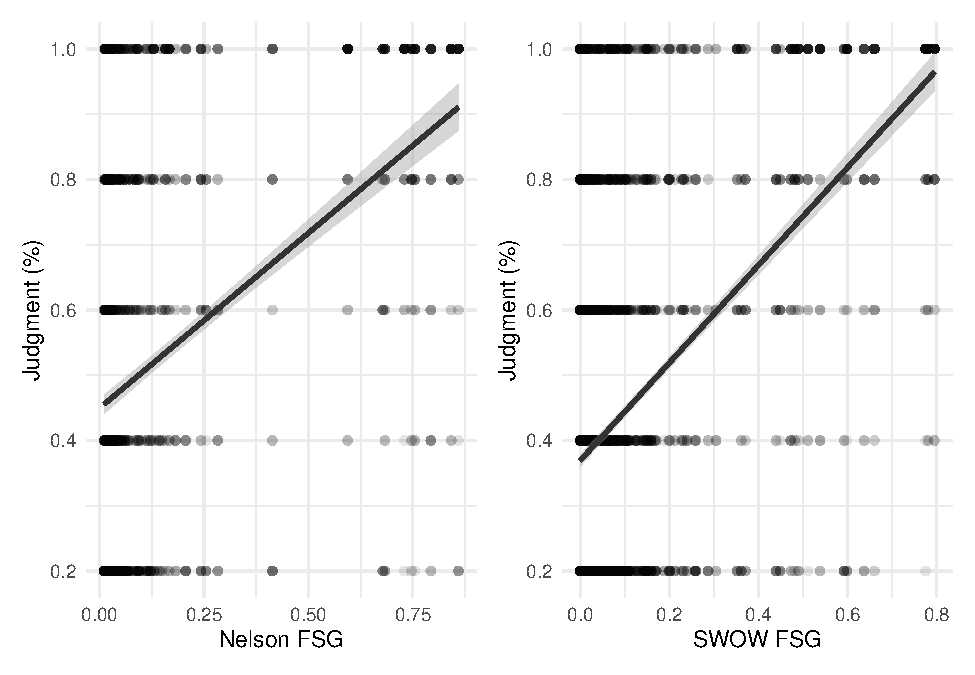
\includegraphics[keepaspectratio]{long-ratings_files/figure-latex/fig-fsg-swow-scores-1.pdf}}
\caption{\label{fig:fig-fsg-swow-scores}Relationship between participants' probability judgments and normative association strength. The left panel shows judgments plotted against Nelson free association forward strength, and the right panel shows judgments plotted against SWOW free association strength. Points represent individual cue--target judgments (scaled to proportions), and lines represent fitted linear regression slopes with 95\% confidence intervals. Participants' judgments increased systematically with both normative measures}
\end{figure}

\subsection{Hypothesis 2}\label{hypothesis-2}

To analyze this hypothesis, we used mixed linear models to predict
participant judgments of association for the experimental, control, and
matched groups. In the experimental group, participants judged their own
free association norms, providing a baseline against which we can
compare group differences for Hypothesis 3. The SWOW norms were used as
the predictor because they offered greater overlap with participant
judgments. The same model structure from Hypothesis 1 was applied, with
random intercepts for participants and random slopes for the free
association predictor.

The experimental norms group showed a biased intercept,
\(\hat{\beta} = 0.66\), 95\% CI \([0.62, 0.70]\), \(t(1431) = 35.54\), \(p < .001\), and a sensitive slope,
\(\hat{\beta} = 0.29\), 95\% CI \([0.24, 0.34]\), \(t(1431) = 10.84\), \(p < .001\), with variability across
participants (\emph{SD} intercept = 0.10, \emph{SD} slope = 0.08). The matched
group, who judged the same pairs as the experimental group, showed
similar results with a biased intercept,
\(\hat{\beta} = 0.57\), 95\% CI \([0.53, 0.62]\), \(t(1431) = 24.91\), \(p < .001\), and a non-zero slope,
\(\hat{\beta} = 0.26\), 95\% CI \([0.20, 0.32]\), \(t(1431) = 8.87\), \(p < .001\) (\emph{SD} intercept = 0.14, \emph{SD}
slope = 0.13). Finally, the control group, who judged parallel
cue--response pairs from the norms database, showed the same pattern of
biased intercepts, \(\hat{\beta} = 0.57\), 95\% CI \([0.54, 0.60]\), \(t(2748) = 34.80\), \(p < .001\), and
significant slopes, \(\hat{\beta} = 0.22\), 95\% CI \([0.19, 0.26]\), \(t(2748) = 11.87\), \(p < .001\) (\emph{SD}
intercept = 0.10, \emph{SD} slope = 0.08). Analyses with the Nelson norms
confirmed the robustness of these results.

These findings replicate prior work (Maki, 2007b, 2007a; Maxwell \& Buchanan, 2020; Valentine \& Buchanan, 2013), showing systematic overestimation
reflected in the bias factor (intercept), which typically falls between
0.40 and 0.60. The experimental group intercept was somewhat higher than
these traditional values, likely reflecting task demands, whereas the
control and matched groups aligned closely with prior findings. All
three groups demonstrated sensitivity to differences in associative
strength, but with shallow slopes (0.20--0.40), consistent with previous
evidence that people are not perfectly sensitive to strength
differences, a pattern also common in the judgments of learning
literature (Koriat, 2008; Koriat \& Bjork, 2006).

\subsection{Hypothesis 3}\label{hypothesis-3}

For our final hypothesis, the bias and sensitivity factors for the
experimental norm group were calculated against their own free
association norms using the same mixed models described above. The bias
factor was lower than the values observed in Hypothesis 2,
\(\hat{\beta} = 0.36\), 95\% CI \([0.31, 0.40]\), \(t(2003) = 14.64\), \(p < .001\) (\emph{SD} = 0.14), while the
sensitivity slope was higher than any of the three slopes from
Hypothesis 2, \(\hat{\beta} = 0.54\), 95\% CI \([0.49, 0.59]\), \(t(2003) = 19.59\), \(p < .001\) (\emph{SD} = 0.13).
Confidence intervals confirmed that these estimates were significantly
different from the previous results. Together, these findings indicate
that when participants judged with respect to their own frequency norms,
they showed reduced bias and greater sensitivity, reflecting improved
calibration of numerical estimates. This pattern supports the idea that
expertise, here operationalized as repeated experience with
self-generated associations, enhances individuals' ability to make
accurate quantitative judgments from memory.

\section{Discussion}\label{discussion}

In viewing these findings, it appears that participants can judge the
associative strength between word--pairs, and they perform especially
well when judging their own associative norms. The experimental group
demonstrated greater accuracy in distinguishing low- and high-frequency
relationships compared to both the matched and control groups. Repeated
interaction with the word--pairs improved performance, suggesting that
expertise supports more accurate quantitative judgments. This outcome is
consistent with a broader literature showing that experts demonstrate
enhanced working memory within their domains (Chase \& Simon, 1973; Ericsson \& Delaney, 1998)
as well as deeper access to long-term memory structures (Ericsson \& Delaney, 1999).
Previous research on judgments of associative memory (JAM) has suggested
that practice and feedback do not always yield improvements (Koriat \& Bjork, 2005; Maki, 2007a); however, this results indicates that experience with one's
own memory is better than experience in practicing judgments with
feedback.

One answer lies in how we frame these tasks as problems of numerical
estimation. Participants were originally asked to judge what 100 college
students would say in response to a cue word, the logic by which free
association norms are defined (Nelson et al., 2000). In effect, JAM tasks are
problems of probability judgment: given a cue, what is the expected
frequency of a particular response? This study revealed that even when
participants generated many unique responses, their judgments still
aligned with normative probabilities, showing that people can
approximate collective likelihoods. This result is hardly surprising,
humans make probability judgments constantly in daily life: estimating
how long a commute will take, whether the stove was turned off, how long
to wait for a late friend, or whether enough studying has been done
before an exam. The popular game show Family Feud capitalized on exactly
this capacity: contestants estimate the most probable answers given a
cue, which would have made for dull television if people were incapable
of such probabilistic reasoning.

At the same time, the results underscore a common challenge in numeracy:
daily practice with estimation does not necessarily make us precise
estimators. Metacognitive research has repeatedly shown that people tend
to overestimate their learning and memory performance (Koriat, 2008; Koriat \& Bjork, 2005, 2006). Similarly, in our study, participants
exhibited systematic bias (intercepts \textgreater{} 0), even when judging their own
norms. Although slopes were steeper in the experimental group than in
the control and matched groups, they remained below 1.0, the benchmark
for perfect sensitivity. Thus, while participants became more calibrated
when judging their own norms, they still showed under-sensitivity to
actual frequencies.

From a broader perspective, these results extend the study of numerical
cognition into the domain of memory judgments. Participants are not
merely retrieving associations but estimating their frequency of
occurrence, a task structurally similar to other probabilistic judgments
in everyday numeracy (Gigerenzer \& Hoffrage, 1995; Reyna et al., 2009). Expertise reduces
bias and enhances sensitivity, but systematic imperfections remain. For
applied contexts, this finding means that encouraging learners to
interact repeatedly with material (much like participants did with
word--pairs here) may improve calibration, but ``foresight bias'' and
overestimation are unlikely to be eliminated entirely (Koriat, 2008).
Future work could profitably examine how stimulus features, such as
baseline word frequency or semantic richness, further shape numeric
estimation from memory, and whether scaffolds from the numeracy
literature (e.g., training in base rates or frequency formats) could
reduce residual bias.

\newpage

\section{References}\label{references}

\setlength{\parindent}{-0.5in}
\setlength{\leftskip}{0.5in}

\phantomsection\label{refs}
\begin{CSLReferences}{1}{0}
\bibitem[\citeproctext]{ref-aust2022}
Aust, F., Barth, M., Diedenhofen, B., Stahl, C., Casillas, J. V., \& Siegel, R. (2022). \emph{Papaja: Prepare american psychological association journal articles with r markdown}. \url{https://CRAN.R-project.org/package=papaja}

\bibitem[\citeproctext]{ref-Buchanan2010}
Buchanan, E. M. (2010). {Access into memory: Differences in judgments and priming for semantic and associative memory}. \emph{Journal of Scientific Psychology}, \emph{March}, 1--8.

\bibitem[\citeproctext]{ref-Chase1973}
Chase, W. G., \& Simon, H. A. (1973). {Perception in chess}. \emph{Cognitive Psychology}, \emph{4}(1), 55--81. \url{https://doi.org/10.1016/0010-0285(73)90004-2}

\bibitem[\citeproctext]{ref-Cutler1989}
Cutler, B. L., \& Wolfe, R. N. (1989). {Self-monitoring and the association between confidence and accuracy}. \emph{Journal of Research in Personality}, \emph{23}(4), 410--420. \url{https://doi.org/10.1016/0092-6566(89)90011-1}

\bibitem[\citeproctext]{ref-dedeyne2019}
De Deyne, S., Navarro, D. J., Perfors, A., Brysbaert, M., \& Storms, G. (2019). The {``}Small World of Words{''} English word association norms for over 12,000 cue words. \emph{Behavior Research Methods}, \emph{51}(3), 987--1006. \url{https://doi.org/10.3758/s13428-018-1115-7}

\bibitem[\citeproctext]{ref-dehaene2011}
Dehaene, S. (2011). \emph{The Number Sense: How the Mind Creates Mathematics, Revised and Updated Edition}. Oxford University Press, USA.

\bibitem[\citeproctext]{ref-Dunning2003}
Dunning, D., Johnson, K., Ehrlinger, J., \& Kruger, J. (2003). {Why People Fail to Recognize Their Own Incompetence}. \emph{Current Directions in Psychological Science}, \emph{12}(3), 83--87. \url{https://doi.org/10.1111/1467-8721.01235}

\bibitem[\citeproctext]{ref-Ericsson1998}
Ericsson, K. A., \& Delaney, P. F. (1998). {Working Memory and Expert Performance}. In K. Gilhooly \& R. H. Logie (Eds.), \emph{Working memory and thinking}. Taylor {\&} Francis. \url{https://doi.org/10.4324/9780203346754_chapter_SIX}

\bibitem[\citeproctext]{ref-Ericsson1999}
Ericsson, K. A., \& Delaney, P. F. (1999). {Long-Term Working Memory as an Alternative to Capacity Models of Working Memory in Everyday Skilled Performance}. In A. Miyake \& P. Shah (Eds.), \emph{Models of working memory} (pp. 257--297). Cambridge University Press. \url{https://doi.org/10.1017/CBO9781139174909.011}

\bibitem[\citeproctext]{ref-Foster2012}
Foster, L. E., \& Buchanan, E. M. (2012). {Judgments of Memory: Do the Number and Presentation of Cues Available Help?} \emph{Journal of Psychological Inquiry}, \emph{17}(2), 17--25.

\bibitem[\citeproctext]{ref-gelman2006}
Gelman, A. (2006). Multilevel (hierarchical) modeling: What it can and cannot do. \emph{Technometrics}, \emph{48}(3), 432--435. \url{https://doi.org/10.1198/004017005000000661}

\bibitem[\citeproctext]{ref-gigerenzer1995}
Gigerenzer, G., \& Hoffrage, U. (1995). How to improve Bayesian reasoning without instruction: Frequency formats. \emph{Psychological Review}, \emph{102}(4), 684--704. \url{https://doi.org/10.1037/0033-295X.102.4.684}

\bibitem[\citeproctext]{ref-Koriat2008}
Koriat, A. (2008). {Alleviating inflation of conditional predictions}. \emph{Organizational Behavior and Human Decision Processes}, \emph{106}(1), 61--76. \url{https://doi.org/10.1016/J.OBHDP.2007.08.007}

\bibitem[\citeproctext]{ref-Koriat2005}
Koriat, A., \& Bjork, R. A. (2005). {Illusions of competence in monitoring one's knowledge during study.} \emph{Journal of Experimental Psychology: Learning, Memory, and Cognition}, \emph{31}(2), 187--194. \url{https://doi.org/10.1037/0278-7393.31.2.187}

\bibitem[\citeproctext]{ref-Koriat2006}
Koriat, A., \& Bjork, R. A. (2006). {Mending metacognitive illusions: a comparison of mnemonic-based and theory-based procedures.} \emph{Journal of Experimental Psychology. Learning, Memory, and Cognition}, \emph{32}(5), 1133--1145. \url{https://doi.org/10.1037/0278-7393.32.5.1133}

\bibitem[\citeproctext]{ref-Maki2007a}
Maki, W. S. (2007a). {Judgments of associative memory}. \emph{Cognitive Psychology}, \emph{54}(4), 319--353. \url{https://doi.org/10.1016/j.cogpsych.2006.08.002}

\bibitem[\citeproctext]{ref-Maki2007}
Maki, W. S. (2007b). {Separating bias and sensitivity in judgments of associative memory.} \emph{Journal of Experimental Psychology. Learning, Memory, and Cognition}, \emph{33}(1), 231--237. \url{https://doi.org/10.1037/0278-7393.33.1.231}

\bibitem[\citeproctext]{ref-maxwell2020}
Maxwell, N. P., \& Buchanan, E. M. (2020). Investigating the interaction of direct and indirect relation on memory judgments and retrieval. \emph{Cognitive Processing}, \emph{21}(1). \url{https://doi.org/10.1007/s10339-019-00935-w}

\bibitem[\citeproctext]{ref-maxwell2021}
Maxwell, N. P., \& Huff, M. J. (2021). The deceptive nature of associative word pairs: the effects of associative direction on judgments of learning. \emph{Psychological Research}, \emph{85}, 1757--1775. \url{https://doi.org/10.1007/s00426-020-01342-z}

\bibitem[\citeproctext]{ref-Nelson2005}
Nelson, D. L., Dyrdal, G. M., \& Goodmon, L. B. (2005). {What is preexisting strength? Predicting free association probabilities, similarity ratings, and cued recall probabilities}. \emph{Psychonomic Bulletin {\&} Review}, \emph{12}(4), 711--719. \url{https://doi.org/10.3758/BF03196762}

\bibitem[\citeproctext]{ref-Nelson2000}
Nelson, D. L., McEvoy, C. L., \& Dennis, S. (2000). {What is free association and what does it measure?} \emph{Memory {\&} Cognition}, \emph{28}(6), 887--899. \url{https://doi.org/10.3758/BF03209337}

\bibitem[\citeproctext]{ref-nelson2004}
Nelson, D. L., McEvoy, C. L., \& Schreiber, T. A. (2004). The University of South Florida free association, rhyme, and word fragment norms. \emph{Behavior Research Methods, Instruments, \& Computers}, \emph{36}(3), 402--407. \url{https://doi.org/10.3758/BF03195588}

\bibitem[\citeproctext]{ref-reyna2008}
Reyna, V. F., \& Brainerd, C. J. (2008). Numeracy, ratio bias, and denominator neglect in judgments of risk and probability. \emph{Learning and Individual Differences}, \emph{18}(1), 89--107. \url{https://doi.org/10.1016/j.lindif.2007.03.011}

\bibitem[\citeproctext]{ref-reyna2009}
Reyna, V. F., Nelson, W. L., Han, P. K., \& Dieckmann, N. F. (2009). How numeracy influences risk comprehension and medical decision making. \emph{Psychological Bulletin}. \url{https://doi.org/10.1037/a0017327}

\bibitem[\citeproctext]{ref-Valentine2013}
Valentine, K. D., \& Buchanan, E. M. (2013). {JAM-boree: An application of observation oriented modelling to judgements of associative memory}. \emph{Journal of Cognitive Psychology}, \emph{25}(4), 400--422. \url{https://doi.org/10.1080/20445911.2013.775120}

\end{CSLReferences}


\end{document}
